\documentclass[12pt,onecolumn,a4paper]{article}
\usepackage{epsfig,graphicx,amsthm,amsmath,amsfonts}
\usepackage{color,xcolor}
\usepackage{pgfplots}
\pgfplotsset{compat=newest}
\usepackage{tikz}
\usepackage{caption}
\usepackage{subcaption}
\usepackage{multirow}
\usepackage{xepersian}
\settextfont{XB Zar}
\setlatintextfont{Times New Roman}

\newtheorem{theorem}{قضیه}[section]
\newtheorem{corollary}{نتیجه‌}[theorem]

\pgfplotstableread[col sep = comma]{gibbs.csv}\gibbs
\pgfplotstableread{
-1 0
-1 -1
0 -1
0 1
1 1
1 0
}\gibbsref
% \pgfplotstableread[col sep = comma]{adv_phenom_oned.txt}\signoned
% \pgfplotstableread[col sep = comma]{adv_phenom_mono.txt}\signmono
% \pgfplotstableread[col sep = comma]{adv_phenom_cheby.txt}\signcheby
% \pgfplotstableread[col sep = comma]{adv_phenom_legen.txt}\signlegen
% \pgfplotstableread[col sep = comma]{adv_phenom_samples.txt}\signmemory

\begin{document}
\title{توجیه وجود مثال‌های خصمانه \\ و انتقال‌پذیری آن‌ها} 
\author{رامین براتی}
\date{\today}
\maketitle

\begin{abstract}
یادگیری عمیق در مرکز پیشرفت‌های اخیر در یادگیری ماشین و هوش مصنوعی قرار دارد. با این که این مدل‌ها توانایی فراانسانی در انجام بعضی کاربردها از خود نشان می‌دهند، مطالعات نشان داده است که این مدل‌ها به تغییرات کوچک و غیر قابل تشخیص در ورودی حساس هستند. این اختلالات را اختلالات خصمانه نام‌گذاری کرده‌اند. پدیده‌ی اختلالات خصمانه تهدید قابل توجهی برای استفاده از مدل‌های یادگیری ماشین در کاربردهای نیازمند ایمنی است و به همین دلیل، تحقیقات بسیاری در این مسیر انجام شده است. در این مقاله، دیدگاه جدیدی در مورد دلیل وجود این پدیده ارائه می‌دهیم. با تکیه بر این دیدگاه، روشی برای ایمن‌سازی شبکه‌های عصبی به حملات خصمانه ارائه می‌دهیم. نتایج اولیه حاکی از موثر بودن روش پیشنهادی در کاهش قابل توجه حساسیت شبکه‌های عصبی به مثال‌های خصمانه است. در عین حال، پیاده‌سازی روش پیشنهادی وابستگی‌ای به شبکه‌های عصبی ندارد و به راحتی قابل انتقال به دیگر مدل‌های یادگیری ماشین نیز هست.
\end{abstract}

\section{مقدمه} 
با پیشرفت‌هایی که اخیرا در الگوریتم‌ها و قدرت محاسباتی به وجود آمده، یادگیری ماشین به یکی از پرکاربردترین ابزارها در صنایع مختلف تبدیل شده است. بدون شک، ظهور و معرفی آموزش عمیق به همراه وجود مجموعه‌های بزرگ آموزشی را می‌توان مسئول بخش قابل توجهی از این پیشرفت‌ها دانست. موفقیت‌ کاربرد آموزش عمیق در مسائل طبقه‌بندی تصاویر، شناسایی اشیا، پردازش زبان طبیعی و دیگر کاربردهای متنوع جایگاه شبکه‌های عصبی چندلایه در صنایع مختلف را نیز تثبیت کرده است.

با توجه به این پیشرفت‌ها، طبیعی است که بخواهیم از این مدل‌ها در کاربردهایی مانند ماشین‌های خودران و دیگر کاربردهایی که امنیت در آنها اهمیت دارد استفاده کنیم. با این حال، در
\cite{szegedy2013intriguing} 
نشان داده شد که مدلهای عمیق به پدیده‌ی مثال‌های خصمانه حساس هستند. مثال‌های خصمانه نقاطی در همسایگی مثال‌های طبیعی هستند که طبقه‌بند در آن نقاط خروجی اشتباه می‌دهد. در بعضی از موارد، تفاوت میان مثال خصمانه با مثال طبیعی برای انسان قابل تشخیص نیست.

انتظار می‌رود که در آینده‌ی نزدیک، مدل‌های عمیق بسیاری در دنیای فیزیکی تعیبیه شوند. در عین حال، مطالعات و تحقیقات اخیر نشان می‌دهند که مثال‌های خصمانه را در دنیای واقعی نیز می‌توان به کار برد. برای مثال، می‌توان ورودی را به گونه‌ای تغییر داد که دستگاه‌هایی که برای گرفتن دستورات از مدل‌های شناسایی گفتار استفاده می‌کنند دستورات اشتباهی را اجرا کنند و یا باعث شد که ماشین‌های خودران در شناسایی عابران پیاده دچار اشتباه شوند. این مسئله، نگرانی‌های بسیاری را در مورد ایمنی استفاده از مدل‌های یادگیری ماشین و شبکه‌های عمیق به وجود آورده است.

در کاربردها، شبکه‌های عصبی عمیق را به صورت مدلهای جعبه سیاه در نظر می‌گیرند. به این معنی که می‌دانیم که این مدل‌ها عملکرد خوبی دارند، ولی به طرز کار درونی آن‌ها وقوف نداریم. دلیل وجود مثال‌های خصمانه یکی از پایه‌ای‌ترین مسائل  مطرح در این زمینه است. با این حال، عدم وجود درک کامل از ساز و کار این مدل‌ها و سختی‌های مرتبط با کار در فضاهای بعد بالا، توضیح و تشریح این دلایل را مشکل کرده است. دلیل وجود این پدیده هنوز یک مسئله‌ی باز است و ما خواننده را به \cite{Yuan_2019} برای مطالعه‌ی بیشتر در مورد این پدیده ارجاع می‌دهیم.

در این مقاله، ما دیدگاه جدیدی در مورد دلیل به وجود آمدن پدیده‌ی مثال‌های خصمانه در شبکه‌های عصبی را ارائه داده و مسیر جدیدی را برای مقابله با تاثیرات این پدیده ارائه می‌کنیم. این مقاله در پنج بخش تنظیم شده است. پس از مقدمه، در بخش دوم، مروری بر تعدادی از دیدگاه‌های ارائه شده‌ی مرتبط با دیدگاه پیشنهادی خواهیم داشت. سپس، در بخش سوم، دیدگاه پیشنهادی را تشریح می‌دهیم. در بخش چهارم، شواهدی  در تایید دیدگاه پیشنهادی ارائه داده و بخش پنجم را نیز به جمع‌بندی و تعیین قدم‌های بعدی در این مسیر اختصاص داده‌ایم.

\section{کارهای مرتبط}
تاکنون، برای وجود مثال‌های خصمانه سه دلیل ارائه شده است. اولین دیدگاه توسط سجدی و همکاران\cite{szegedy2013intriguing}
مطرح شد. این دیدگاه، که با نام دیدگاه پاکت‌های نادر شناخته می‌شود، به شرح زیر است. در این دیدگاه، دلیل وجودی مثال‌های خصمانه وجود پاکت‌هایی در فضای ورودی شبکه هستند که احتمال مشاهده‌ی آنها بسیار کم است و شبکه در آن نواحی خروجی مناسبی نمی‌دهد. در این دیدگاه رابطه‌ی مثال‌های خصمانه با فضای ورودی شبکه را مشابه رابطه‌ی میان اعداد گویا و اعداد حقیقی می‌دانند. به این معنی که، احتمال گویا بودن یک نمونه‌ی تصادفی از یک بازه از اعداد حقیقی صفر است، با این وجود در همسایگی هر عدد حقیقی عددی گویا یافت می‌شود. با این حال،
همان گونه که در
\cite{tanay2016boundary}
نیز به آن اشاره شده است، دلیل محکمی برای نشان دادن چنین رفتاری توسط شبکه ارائه نشده است و صرفا به مرتبط کردن آن به بسیار غیرخطی بودن نمایش یادگیری شده توسط شبکه اکتفا شده است. در 
\cite{Tabacof_2016}
 نیز شواهدی ارائه شده است که طبق این شواهد، مثال‌های خصمانه الزاما به صورت ایزوله در فضا پخش نمی‌شوند و نواحی چگال و فشرده‌ای از این مثال‌ها نیز وجود دارد. این دیدگاه چگونگی انتقال این مثال‌ها به شبکه‌های دیگر را نیز مشخص نمی‌کند.

دیدگاه دوم توسط گودفلو و همکاران\cite{goodfellow2014explaining}
مطرح شده است. این دیدگاه با نام دیدگاه خطی بودن شناخته می‌شود. طبق این دیدگاه، پدیده‌ی مثال‌های خصمانه در طبقه‌بندهای خطی در ابعاد بالا ظهور می‌کند و دلیل مشاهده‌ی این پدیده در شبکه‌های عصبی نیز مرتبط با علاقه‌ی ما در استفاده از الگوهای خطی در مدلسازی و آموزش این شبکه‌ها می‌باشد. گودفلو و همکاران با استفاده از این دیدگاه حمله‌ی
\lr{FGSM}
را طراحی کردند که از این خطی بودن شبکه‌های عصبی برای تولید مثال‌های خصمانه استفاده می‌کند. ضرب داخلی بین یک بردار وزن $w$ و یک مثال خصمانه‌ی $\tilde{x}=x+\eta$ را در نظر بگیرید.
\begin{equation*}
w^T\tilde{x}=w^Tx+w^T\eta
\end{equation*}
طبق معادله، اگر $\eta$ را برابر با $\mathrm{sign}(w)$ در نظر بگیریم، بیشترین تغییر را، تحت قید نورم ماکزیموم، در خروجی اعمال کرده‌ایم. خطی بودن به این معناست که شبکه رفتاری مشابه از خود نشان داده و در صورتی که $\eta$ را برابر با علامت گرادیان تابع هزینه در نقطه‌ی $x$ قرار دهیم، شبکه در طبقه‌بندی دچار خطا خواهد شد.

طبق این دیدگاه، دلیل انتقال مثال‌های خصمانه به دیگر شبکه‌ها، همگرایی این مدل‌ها به طبقه‌بند خطی بهینه است. دیدگاه خطی بودن دو پیش بینی مستقیم دارد، اول این که تمامی طبقه‌بندهای خطی از پدیده‌ی مثال‌های خصمانه رنج می‌برند و دوم این که اثر خطی بودن با افزایش ابعاد مسئله تشدید می‌شود. با این وجود، در
\cite{tanay2016boundary}
هر دوی این پیش‌بینی‌ها زیر سوال می‌روند. ابتدا مسئله‌ای  مصنوع را در نظر می‌گیرند که برای آن طبقه‌بندی خطی وجود دارد که از مثال‌های خصمانه آزاد است و در ادامه نشان می‌دهند که در یک مسئله‌ی واقعی نیز با افزایش ابعاد قدرت مثال‌های خصمانه تشدید نمی‌شود.

دیدگاه سوم توسط تانای و همکاران
\cite{tanay2016boundary}
 و با نام دیدگاه کجی مرز ارائه شده است. این دیدگاه برای طبقه‌بندهای خطی پیشنهاد شده و ظهور آن در شبکه‌های عصبی را منتج از شکلی غیرخطی از این پدیده می‌دانند. یک مسئله‌ی طبقه‌بندی دو کلاسی را در نظر بگیرید که برای آن یک طبقه‌بند خطی را آموزش داده‌ایم. این طبقه‌بند خطی یک مرز تصمیم
 $c$
 برای جدا کردن دو کلاس می‌یابد. حال طبقه‌بند بهینه‌ای را برای همان مسئله در نظر بگیرید که توسط مرکزهای دو کلاس تعریف شده باشد. این طبقه‌بند نیز یک مرز تصمیم
 $c^*$
 برای جدا کردن دو کلاس تعریف می‌کند. طبق دیدگاه کجی مرز در صورتی که مرز
 $c$
 با
 $c^*$
 زاویه داشته باشد، برای طبقه‌بند مثال‌های خصمانه وجود خواهد داشت. تانای و همکاران در ادامه نشان می‌دهند که می‌توان زاویه‌ی بین دو مرز را با منظم کردن\LTRfootnote{regularize}
طبقه‌بند کاهش داد. در پایان، تانای و همکاران با توجه به نوع و شکل اختلالات خصمانه‌ای که در شبکه‌های عصبی مشاهده می‌کنند، دلیل وجود مثال‌های خصمانه برای این شبکه‌ها را منظم نبودن این شبکه‌ها اعلام می‌کنند. با این که تانای و همکاران دلایل خوبی در تایید دیدگاه کجی مرز ارائه می‌دهند، چگونگی تعمیم آن به شبکه‌های عصبی و دیگر مدل‌های غیرخطی را مشخص نمی‌کنند. همچنین، در این دیدگاه دلیلی برای انتقال‌پذیری مثال‌های خصمانه ارائه نشده است.

وجود این ناسازگازی‌ها محققان را به سمت ارائه‌ی توجیهات دیگری سوق داده است. گروهی از محققان دلیل وجود این پدیده را با ویژگی‌های مورد استفاده در طبقه‌بندی مرتبط می‌کنند. به طور مثال، در \cite{eykholt2019robust} شبکه را با استفاده از دودویی سازی ورودی نسبت به مثال‌های خصمانه مقاوم کردند. یا در \cite{ilyas2019adversarial} دلیل وجود مثال‌های خصمانه را حضور ویژگی‌های ناپایداری می‌دانند که با برچسب خروجی همبستگی دارند. این مطالعات نشان می‌دهند که وجود مثال‌های خصمانه با داده‌های آموزشی استفاده شده و طبقه‌بند هدف ارتباط تنگاتنگی دارد. با این وجود، در حال حاضر، چارچوب یکپارچه‌ای برای توجیه و توصیف این رابطه ارائه نشده است.

همان گونه که مشاهده می‌شود، هیچ‌کدام از دیدگاه‌های مطرح شده توانایی توجیه و تشریح تمامی مشاهدات مرتبط با مثال‌های خصمانه را ندارند. با این حال، هرکدام بخش محدودی از مشاهدات را توجیه می‌کنند. در اینجا، دیدگاه جدیدی را مطرح می‌کنیم که توانایی توجیه وجود مثال‌های خصمانه و انتقال‌پذیری آن‌ها را دارد و  در عین حال، با مشاهداتی که توسط دیدگاه‌های قبلی مطرح شده نیز سازگازی دارد. در ادامه، این دیدگاه جدید را شرح می‌دهیم.

\section{تکینگی‌ها و مثال‌های خصمانه}
در این بخش، دیدگاه جدیدی را در مورد دلیل وجود مثال‌های خصمانه و انتقال‌پذیری آن‌ها ارائه می‌دهیم. در این دیدگاه وجود مثال‌های خصمانه و انتقال‌پذیری آنها نتیجه‌ی وجود تکینگی در تابع هدف به همراه وجود الگوهای فرکانس بالا در سیگنال ورودی در نظر گرفته می‌شود. مشخصه‌ی مهم مثال‌های خصمانه انتقال‌پذیری آنهاست. در اینجا، انتقال‌پذیری مثال‌های خصمانه را نتیجه‌ی غیرمستقیم اصل داربو در مورد تکینگی‌ها و بسط‌های طیفی در نظر می‌گیریم.

قبل از شرح دیدگاه پیشنهادی منظورمان از تکینگی و الگوهای فرکانس بالا را مشخص می‌کنیم. در اینجا از تعریف عام تکینگی استفاده می‌کنیم، به این معنی که ناپیوستگی‌های تابع نیز، به همراه قطب‌ها و ...، به عنوان تکینگی  در نظر گرفته می‌شوند. اگر تبدیل نمونه‌ی ورودی را در دامنه‌ی فرکانس در نظر بگیریم، الگوهای فرکانس بالا را می‌توان با اعمال یک  فیلتر بالا گذر به دست آورد.

ابتدا، با یک مثال، چگونگی به وجود آمدن مناطق خصمانه را توجیه می‌کنیم. پس از آن به شرح دقیق‌تری از مشکل مثال‌های خصمانه خواهیم پرداخت. در این راستا، یک مسئله‌ی طبقه‌بندی تعریف می‌کنیم. فرض کنید که قصد یادگیری یک طبقه‌بند برای تشخیص اعداد مثبت و منفی در بازه‌ی 
$[-1,1]$ 
را داشته باشیم. در نتیجه، تابعی که قصد یادگیری آن را داریم تابع 
$f(x)=\mathrm{sign}(x)$ 
است. همان گونه که در شکل \ref{fig:1d} نیز مشاهده می‌شود، تابع 
$f$ 
در نقطه‌ی مرکز مختصات یک ناپیوستگی دارد. برای آموزش شبکه به یک مجموعه‌ی داده نیاز خواهیم داشت. به این منظور، بازه‌ی 
$[-1,1]$ 
را به بازه‌های هم اندازه افراز کرده و نقاط پایانی این بازه‌ها را به عنوان مجموعه‌ی نمونه‌های آموزشی در نظر می‌گیریم.

\begin{figure}
	\centering
	\begin{subfigure}[b]{0.45\textwidth}
		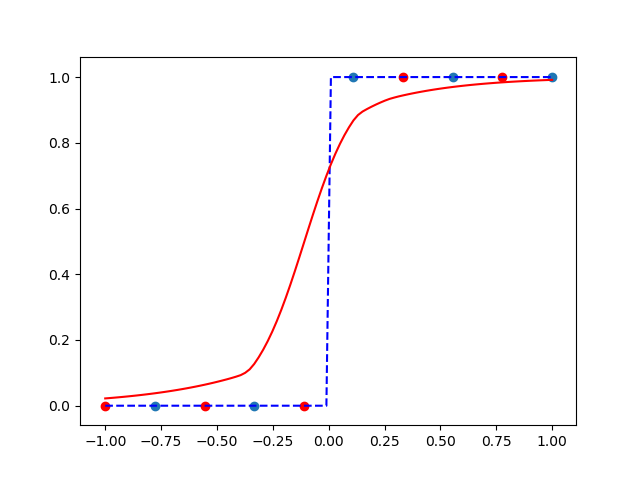
\includegraphics[width=\textwidth]{1d_plain.png}
		\caption{نمونه‌های تک بعدی}
		\label{fig:1dplain}
	\end{subfigure}
	~ %add desired spacing between images, e. g. ~, \quad, \qquad, \hfill etc. 
	%(or a blank line to force the subfigure onto a new line)
	\begin{subfigure}[b]{0.45\textwidth}
		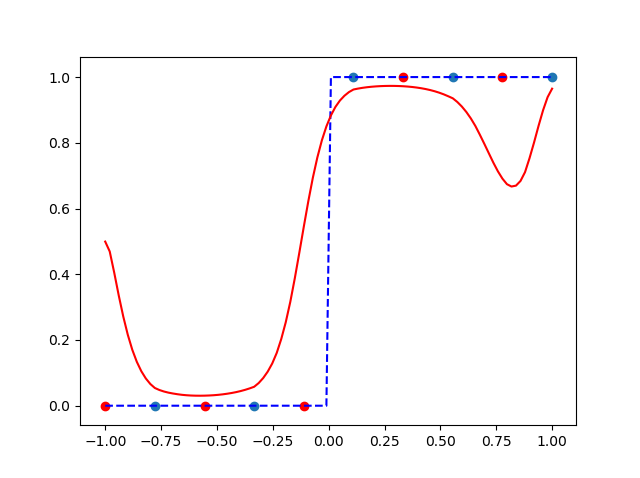
\includegraphics[width=\textwidth]{1d_aug.png}
		\caption{نمونه‌های افزایش بعد یافته}
		\label{fig:1daug}
	\end{subfigure}
	~ %add desired spacing between images, e. g. ~, \quad, \qquad, \hfill etc. 
	%(or a blank line to force the subfigure onto a new line)
	\caption{
		خروجی یک شبکه عصبی کاملا متصل پس از آموزش با نمونه‌های آموزشی تک بعدی و نمونه‌های افزایش بعد یافته. همان گونه که مشاهده می‌شود، در صورت افزایش بعد فرآیند آموزش به شبکه‌ی مورد نظر همگرا نمی‌شود. نقاط آبی نمونه‌های آموزشی و نقاط قرمز نمونه‌های آزمایشی هستند.
	}
	\label{fig:1d}
\end{figure}

همان گونه که در شکل \ref{fig:1dplain} مشاهده می‌شود، فرآیند آموزش در یافتن تابع مورد نظر موفق است و ناپیوستگی در مرکز مختصات نیز صاف شده است. با این وجود، مجموعه‌ی آموزشی را به گونه‌ای می‌توان تغییر داد که فرآیند آموزش در یافتن تابع مورد نظر موفق نباشد. در این راستا، ابعاد ورودی را با استفاده از توابع  پایه‌ی چبیشف افزایش می‌دهیم. در شکل \ref{fig:1daug} نتیجه‌ی آموزش پس از افزایش ابعاد ورودی با 5 پایه‌ی اول چبیشف نشان داده شده است. همان طور که در شکل نیز مشاهده می‌شود، اضافه کردن این ابعاد باعث به وجود آمدن نوساناتی در خروجی شبکه می‌شود. در مقابل، خروجی شبکه در منطقه‌ی اطراف تکینگی به مقدار واقعی تابع نزدیک‌تر شده است. در واقع، برای جبران خطای شبکه در نزدیکی نقطه‌ی تکینگی، شبکه به الگوهای فرکانس بالا نیز حساس شده و این مسئله باعث به وجود آمدن نوسنات در خروجی شبکه می‌شود. البته لازم به ذکر است که فرآیند آموزش در یافتن همبستگی بین ابعاد جدید و خروجی دچار اشتباه نشده است. در حقیقت، با به دست آوردن بسط چبیشف تابع $\mathrm{sign}(x)$ می‌توان دید که ضرایب هیچ‌کدام از پایه‌های فرد چبیشف صفر نیستند.

هم اکنون، پدیده‌ی پیشنهادی را در سناریوی واقعی‌تری بررسی می‌کنیم. در این مثال، هدف ما شبیه‌سازی کاربرد برچسب‌زنی تصاویر است. در این کاربرد، دامنه‌ی ورودی ابرمکعب $[-1,1]^D$ 
است که $D$ در آن تعداد ابعاد ورودی است. نکته‌ای که این مسئله را از سناریوی قبلی متفاوت می‌کند این است که تمامی اطلاعات مورد نیاز برای طبقه‌بندی روی مرز دامنه‌ی ورودی قرار دارد. این موضوع نتیجه‌ی این واقعیت است که برچسب تصویر در صورت نورمال کردن تصویر تغییر نمی‌کند. علاوه بر آن، طبقه‌بندی که تصاویر را برچسب‌زنی می‌کند، عموما، تابعی زوج است. به این معنی که برچسب نمونه نگاتیو شده با نمونه طبیعی برابر است.

قرار داشتن مثال‌های طبیعی بر روی مرز ورودی در مورد تمامی کاربردهای با ابعاد بالا کم و بیش صادق است. این موضوع ناشی از این واقعیت هندسی است که اکثر جرم یک توپ چندین بعدی در نوار نازکی در نزدیکی محیط توپ قرار دارد. این واقعیت را می‌توان با محاسبه‌ی حجم کره در ابعاد بالا نشان داد. در حقیقت، در صورتی که تعداد ابعاد به بی‌نهایت نزدیک شود، حجم کره به صفر میل می‌کند. این موضوع به این معنی است که در صورت نمونه‌براری یکنواخت از درون ابرمکعب یکه بی‌نهایت بعدی، تمامی نمونه‌ها به احتمال قریب به یقین خارج از کره‌ی یکه‌ی بی‌نهایت بعدی هستند.

در این مثال، مسئله‌ی طبقه‌بندی را روی دیسک واحد دو بعدی تعریف می‌کنیم. در این صورت، هر نقطه‌ی دامنه‌ی ورودی را می‌توان با مختصات قطبی $(\rho,\theta)$ 
 نشان داد که در آن $\rho \in [0,1]$ و $\theta \in [-\pi,\pi]$ است. 
 تابع هدف طبقه‌بندی را $f(\rho,\theta)=\mathrm{sign}(\sin \theta)$ در نظر می‌گیریم.
همان طور که گفته شد، در این مثال قصد داریم که مثال‌های آموزشی روی مرز دامنه‌ی ورودی قرار داشته باشند. به این منظور، مجموعه‌ی مثال‌های آموزشی را با افراز محیط دیسک واحد به کمان‌های مساوی تشکیل می‌دهیم. بردار ویژگی برای این مجموعه را با استفاده از مختصات کارتزی نمونه‌ها، یعنی $(x,y)=(\rho\sin\theta,\rho\cos\theta)$، تعریف می‌کنیم. نتیجه‌ی آموزش شبکه روی این مجموعه‌ی آموزشی در شکل مشاهده می‌شود.

\begin{figure}
	\centering
	\begin{subfigure}[b]{0.45\textwidth}
		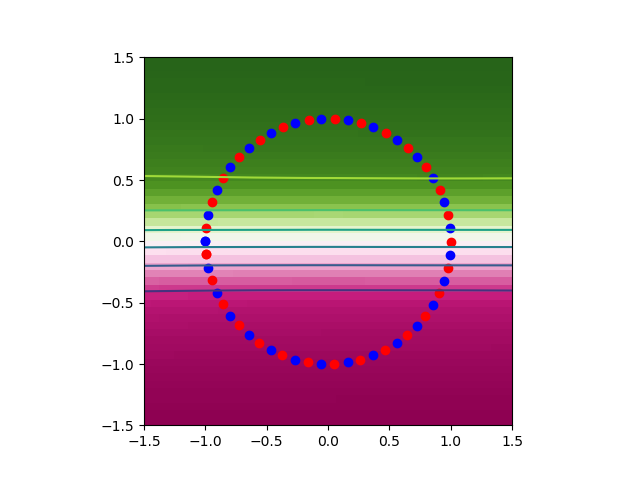
\includegraphics[width=\textwidth]{2d_plain.png}
		\caption{نمونه‌های دو بعدی}
		\label{fig:2dplain}
	\end{subfigure}
	~ %add desired spacing between images, e. g. ~, \quad, \qquad, \hfill etc. 
	%(or a blank line to force the subfigure onto a new line)
	\begin{subfigure}[b]{0.45\textwidth}
		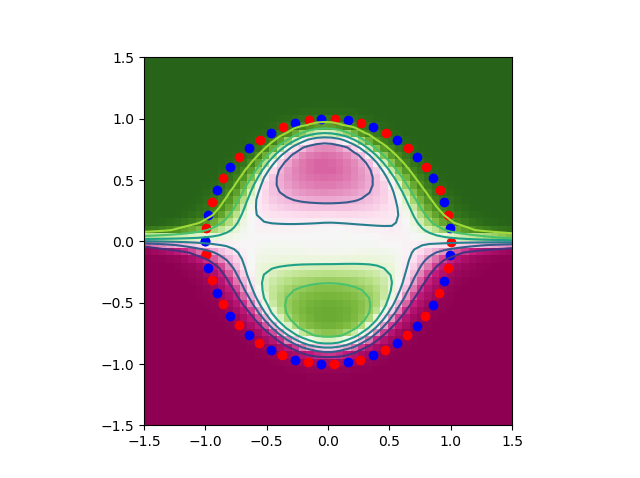
\includegraphics[width=\textwidth]{2d_aug.png}
		\caption{نمونه‌های افزایش بعد یافته}
		\label{fig:2daug}
	\end{subfigure}
	~ %add desired spacing between images, e. g. ~, \quad, \qquad, \hfill etc. 
	%(or a blank line to force the subfigure onto a new line)
	\caption{
		خروجی یک شبکه عصبی کاملا متصل پس از آموزش با نمونه‌های آموزشی دو بعدی و نمونه‌های افزایش بعد یافته روی دیسک یکه. تمامی نمونه‌های آموزشی روی دایره‌ی یکه قرار دارند. در حالت افزایش بعد یافته، ناحیه‌های خصمانه در همسایگی دایره‌ی یکه به وجود آمده است.
	}
	\label{fig:2d}
\end{figure}

مانند مثال قبلی، در اینجا نیز شبکه موفق به یافتن تابع هدف می‌شود. با این حال، مشابه سناریوی پیشین، ابعاد را به گونه‌ای می‌توان افزایش داد که فرآیند آموزش در یافتن طبقه‌بند هدف شکست خورده و متعاقبا مناطق خصمانه به وجود آیند. این بار اما، از چندجمله‌ای‌های پایه‌ی زرنیکه\LTRfootnote{Zernike polynomials} برای افزایش ابعاد استفاده می‌کنیم. به این منظور، ابعاد ورودی را با استفاده از پایه‌های درجه‌ی دو و سه از چندجمله‌ای‌های زرنیکه افزایش می‌دهیم که در مجموع بردار ویژگی را از 2 بعد به 9 بعد افزایش می‌دهد. نتیجه‌ی آموزش شبکه با استفاده از مجموعه‌ی آموزشی افزایش بعد یافته را در شکل \ref{fig:2daug} نشان داده‌ایم. همان گونه که در شکل نیز مشخص است، شبکه روی مرز دیسک مقدار صحیحی خروجی می‌دهد ولی اگر از مرز به سمت مرکز دیسک حرکت کنیم، برچسب ورودی قبل از عبور از مرز تصمیم واقعی تغییر می‌کند. در عمل تمامی نقاط ناحیه‌ی درونی دیسک به اشتباه برچسب زده شده‌اند. در مقابل، اگر از مرز به سمت بیرون دیسک حرکت کنیم، مثال خصمانه نخواهیم یافت.

با توجه به این مشاهده که شبکه بر روی مرز مقدار صحیح را خروجی می‌دهد، می‌توان روشی برای حذف نواحی خصمانه پیشنهاد داد. در صورتی که بتوانیم خروجی شبکه بر روی مرز را به درون توپ یکه تعمیم دهیم، مناطق خصمانه از بین خواهند رفت. از این رو، ورودی را به بازه‌ی $[-1,1]$ منتقل کرده و سپس تبدیل $\tanh(\frac{1}{x})$ را به تک تک ابعاد ورودی اعمال می‌کنیم. در بخش آزمایش‌ها نتیجه‌ی تغییر پیشنهادی بر عملکرد شبکه را مورد بررسی قرار می‌دهیم. 

\section{نواحی خصمانه و ارتباط آن با توزیع مثال‌های آموزشی}
با توجه به نوع مسائل ساختگی و روشی که برای افزایش ابعاد در آنها استفاده کردیم، ممکن است بگوییم که نواحی خصمانه هنگامی که یک طبقه‌بند خطی نیز عملکرد خوبی روی مثال‌های آموزشی دارد به وجود می‌آیند. در این صورت مشاهداتی که در بخش قبل ارائه شدند را می‌توان شاهدی برای دیدگاه خطی بودن نیز در نظر گرفت. در ادامه نشان می‌دهیم که ماهیت وجودی نواحی خصمانه بسیار تحت تاثیر توزیع نمونه‌های آموزشی است و در نتیجه پدیده‌ی مشاهده شده را نمی‌توان ناشی از خطی بودن طبقه‌بند آموزش دیده دانست.

همان گونه که در بخش قبل نیز نشان دادیم، فرآیند آموزش در شناسایی وجود همبستگی بین خروجی و الگوهای فرکانس بالا اشتباه نکرده است. با این حال، همان گونه که در شکل \ref{fig:2daug} نیز مشاهده می‌شود، شبکه در شناسایی رابطه‌ی بین خروجی و اندازه‌ی الگوی ورودی، یعنی $\rho$، دچار خطا شده است. در حقیقت، انتظار ما این است که خروجی شبکه از اندازه‌ی ورودی مستقل باشد ولی فرآیند آموزش به اشتباه بین اندازه‌ی الگوی ورودی و خروجی طبقه‌بند همبستگی پیدا کرده است.

این موضوع، ما را بر آن داشت که تاثیر توزیع‌های متفاوت $\rho$ بر فرآیند آموزش را بررسی کنیم. همان گونه که توضیح دادیم، در مسئله‌ی ساختگی دو بعدی، مثال‌های آموزشی را روی دایره‌ی یکه در نظر گرفتیم. در نتیجه، توزیع $\rho$ تکین بوده و مقدار $\rho$ همیشه برابر با یک است. با این حال، به  جای توپ $l_2$، یا همان دایره‌ی یکه، می‌توان از مکان هندسی توپ‌های دیگر $l_p$ نیز استفاده کرد.

بدین منظور، دو مسئله‌ی جدید با استفاده از توپ‌های $l_1$ و $l_\infty$ تعریف می‌کنیم. بقیه‌ی شرایط مشابه با تعریف ارائه شده در قبل است. توپ $l_1$ مکان هندسی نقاطی است که در رابطه‌ی $\|x\|_1=1$ صدق کنند. به طور مشابه، توپ $l_\infty$ نیز مکان هندسی نقاطی است که در رابطه‌ی $\|x\|_\infty=1$ صدق می‌کنند. در دو بعد، این روابط به شکل زیر هستند.
\[
\|x\|_1=|x_1|+|x_2|=1, \quad \|x\|_\infty=\max(x_1, x_2)=1
\]

\begin{figure}
	\centering
	\begin{subfigure}[b]{0.45\textwidth}
		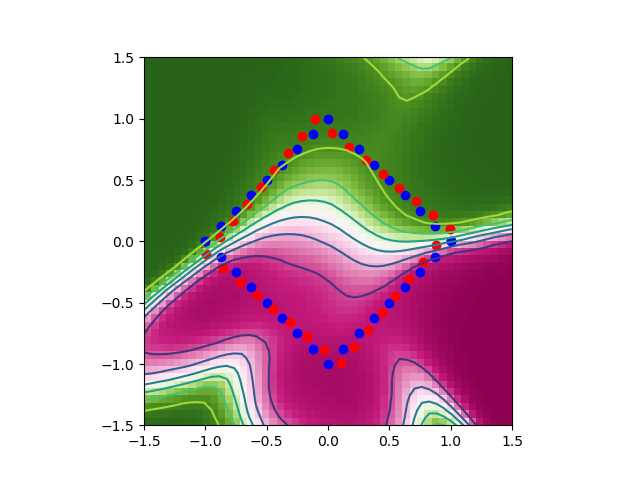
\includegraphics[width=\textwidth]{2d_l1.png}
		\caption{توپ $l_1$}
		\label{fig:ball1}
	\end{subfigure}
	~ %add desired spacing between images, e. g. ~, \quad, \qquad, \hfill etc. 
	%(or a blank line to force the subfigure onto a new line)
	\begin{subfigure}[b]{0.45\textwidth}
		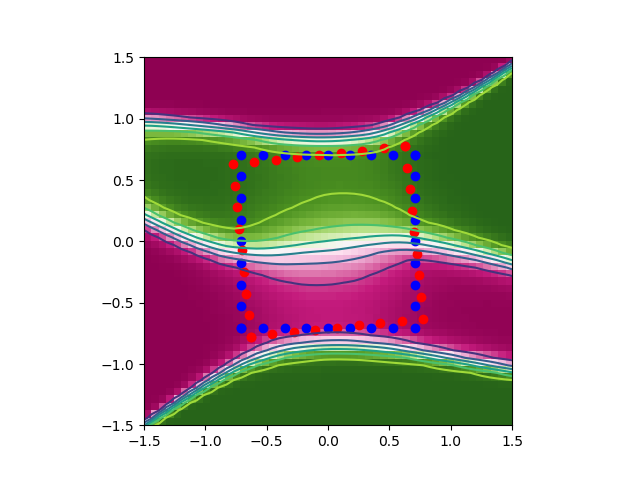
\includegraphics[width=\textwidth]{2d_linf.png}
		\caption{توپ $l_\infty$}
		\label{fig:ballinf}
	\end{subfigure}
	~ %add desired spacing between images, e. g. ~, \quad, \qquad, \hfill etc. 
	%(or a blank line to force the subfigure onto a new line)
	\caption{
		خروجی یک شبکه عصبی کاملا متصل پس از آموزش با نمونه‌های آموزشی دو بعدی افزایش بعد یافته روی دیسک یکه. نقاط آبی نمونه‌های آموزشی و نقاط قرمز، نمونه‌های آزمایشی هستند.
	}
	\label{fig:balls}
\end{figure}

طبقه‌بندهای یافت شده برای این دو توپ را در شکل \ref{fig:balls} نشان داده‌ایم. همان طور که در شکل نیز مشاهده می‌شود، انتخاب توزیع $\rho$ تاثیر قابل توجهی روی نتیجه‌ی فرآیند آموزش شبکه دارد. همان گونه که در شکل \ref{fig:ball1} نیز مشاهده می‌شود، در صورت استفاده از توپ $l_1$، نواحی خصمانه‌ای مشابه با توپ $l_2$ به وجود نیامده، ولی، در مناطق درونی، مرز تصمیم به نمونه‌های آموزشی نزدیک شده است. در مقابل، در صورت استفاده از توپ $l_\infty$، مرز تصمیم در نواحی خارج توپ به نمونه‌ها نزدیک شده است.

می‌توان نشان داد که رفتار فوق برای انتخاب‌های دیگر طبقه‌بند هدف نیز تکرار می‌شود. سناریوی مشابه را با طبقه‌بند هدف 
$f(\rho,\theta)=\mathrm{sign}(\sin2\theta)$ 
در نظر بگیرید. نتیجه‌ی آموزش در این حالات را در شکل \ref{fig:evenballs} نشان داده‌ایم. همان طور که در شکل نیز مشاهده می‌شود، مرز تصمیم، در صورت استفاده از توپ $l_\infty$ از نمونه‌های آموزشی دور بوده و در مقابل در صورت استفاده از توپ $l_1$ مرز به اکثر نمونه‌های آموزشی نزدیک است. در حالت $l_2$، از آنجایی که تابع هدف یکی از پایه‌های درجه دوی زرنیکه است، پایه $Z_{-2}^{2}$ را از ابعاد ورودی حذف می‌کنیم. همان گونه که مشاهده می‌شود، نواحی خصمانه در این حالت نیز به وجود خواهند آمد.

\begin{figure}
	\centering
	\begin{subfigure}[b]{0.3\textwidth}
		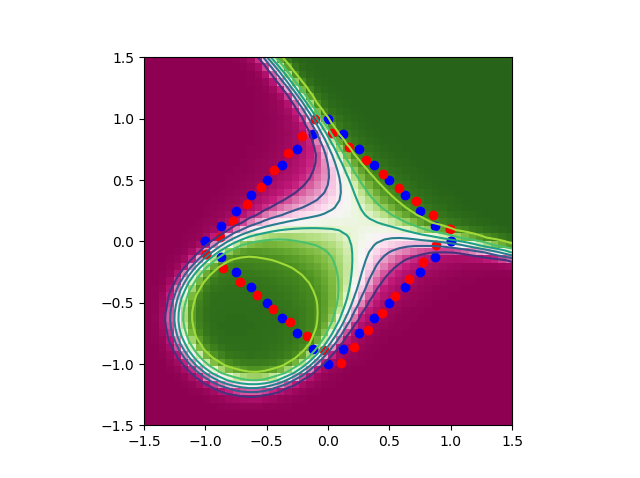
\includegraphics[width=\textwidth]{2d_even_l1.png}
		\caption{توپ $l_1$}
		\label{fig:evenball1}
	\end{subfigure}
	~ %add desired spacing between images, e. g. ~, \quad, \qquad, \hfill etc. 
	%(or a blank line to force the subfigure onto a new line)
	\begin{subfigure}[b]{0.3\textwidth}
		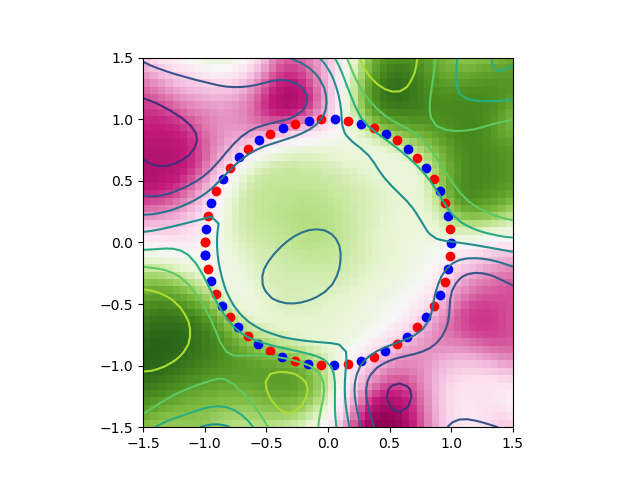
\includegraphics[width=\textwidth]{2d_even_l2.png}
		\caption{توپ $l_2$}
		\label{fig:evenballinf}
	\end{subfigure}
	~ %add desired spacing between images, e. g. ~, \quad, \qquad, \hfill etc. 
	%(or a blank line to force the subfigure onto a new line)
	\begin{subfigure}[b]{0.3\textwidth}
		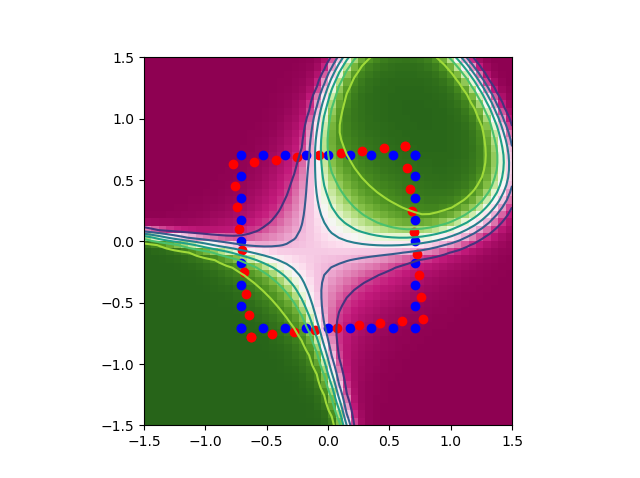
\includegraphics[width=\textwidth]{2d_even_linf.png}
		\caption{توپ $l_\infty$}
		\label{fig:evenballinf}
	\end{subfigure}
	~ %add desired spacing between images, e. g. ~, \quad, \qquad, \hfill etc. 
	%(or a blank line to force the subfigure onto a new line)
	\caption{
		نتیجه‌ی فرآیند آموزش پس از تغییر تابع هدف به $\mathrm{sign}(\sin2\theta)$. همان طور که در نمودارها دیده می‌شود، انتخاب توزیع $\rho$ تاثیر بسزایی در تعیین وجود و نوع نواحی خصمانه در طبقه‌بند یافت شده دارد.
	}
	\label{fig:evenballs}
\end{figure}

نتایج حاصله نشان می‌دهند که به وجود آمدن نواحی خصمانه بیشتر از آنکه به جزییات آموزش و مدل انتخابی مرتبط باشد، ناشی از خواص هندسی سطحی است که نمونه‌های آموزشی روی آن قرار دارند. در حقیقت، به نظر می‌رسد که به وجود آمدن نواحی خصمانه خود تاثیر جانبی پدیده‌ی کلی‌تری در فرآیند آموزش یا ساخت شبکه‌های عصبی هستند.

پدیده‌های مشابه برای چندجمله‌ای‌ها نیز وجود دارد. عملکرد شبکه‌ی عصبی در نواحی خصمانه شباهت قابل توجهی با پدیده‌های رونگه و گیبس دارد. در پدیده‌ی رونگه، توزیع نقاط درون‌یابی نقش حیاتی را در تولید نوسانات در خروجی بازی می‌کند و در پدیده‌ی گیبس وجود ناپیوستگی در تابع هدف باعث به وجود آمدن نوسانات در تقریب ما از تابع خواهد داشت. در حقیقت، نتایج حاصله نشان از وجود رابطه‌‌ای مهم بین تئوری تقریب جهانی برای شبکه‌های عصبی، تئوری تقریب وایرشتراس برای چندجمله‌ای‌ها و نواحی خصمانه دارد.

\section{شواهد و آزمایش‌ها}
در این بخش، شواهدی در تایید رابطه‌ی پدیده‌ی مثال‌های خصمانه و دیدگاه پیشنهادی را ارائه می‌دهیم. همان گونه که در بخش قبل به آن اشاره شد، طبق دیدگاه پیشنهادی، دو روش عمده‌ی مقابله با پدیده‌ی مثال‌های خصمانه منظم‌سازی و روش کمترین مربعات است. با این  حال، وجود این رابطه را بدون استفاده از روش‌های اشاره شده نیز می‌توان نشان داد. با تکیه بر دیدگاه پیشنهادی، هنگام طبقه‌بندی تصاویر با استفاده از شبکه‌های عصبی، می‌توان قید بسیار قویی به شبکه اضافه کرد که شبکه را نسبت به تمامی حملات مبنی بر شهود گرادیان  شبکه، از جمله حمله‌ی \lr{FGSM}، ایمن کند.

می‌دانیم که، در کاربرد طبقه‌بندی تصاویر، دامنه‌ی ورودی شبکه ابرمکعب $[-1,1]^D$ است و $D$ بعد ورودی را نشان می‌دهد. در این کاربرد، می‌توان فرض کرد که برچسب هر نقطه با برچسب نزدیکترین نقطه روی سطح ابرمکعب برابر است. نزدیک‌ترین نقطه روی سطح ابرمکعب به مثال طبیعی را می‌توان با نورمال کردن مقادیر پیکسل‌ها، به گونه‌ای که بزرگترین مقدار مطلق پیکسل‌ها برابر با یک شود به دست آورد. در داده‌های آموزشی ساده‌تر، مانند 
\lr{MNIST}، 
می‌توان فرض کرد که برچسب هر نقطه‌ی روی سطح ابرمکعب با برچسب نزدیکترین گوشه برابر است. در نتیجه، تعداد مثال‌های طبیعی حداکثر به تعداد گوشه‌های این ابرمکعب، یعنی $2^D$ است. طبق دیدگاه پیشنهادی، پدیده‌ی مثال‌های خصمانه ناشی از همگرایی نقطه‌ای شبکه‌ها‌ی یافت شده به میانگین شبکه‌های درون‌یاب گذرنده از این گوشه‌ها است. در این صورت، شبکه‌ای که بر روی مثال‌های طبیعی آموزش داده شده است،  طبقه‌بند خوبی برای نزدیک‌ترین گوشه‌ها به مثال‌های طبیعی خواهد بود. 

 این موضوع را به راحتی می‌توان آزمایش کرد. آزمایش نشان می‌دهد که عملکرد شبکه‌ها بر روی نزدیک‌ترین گوشه‌ها به مثال‌های آموزشی، با حاشیه‌ی بسیار کوچکی، تقریبا برایر با عملکرد شبکه بر روی مثال‌های طبیعی آموزشی است. فقط برچسب تعداد کمی از مثال‌های طبیعی پس از این جابه‌جایی تغییر می‌کند و تصاویر گوشه‌ای که برچسب آنها تغییر می‌کند مثال‌های خصمانه‌ای برای این مثال‌های طبیعی هستند. این مثال‌های خصمانه را می‌توان ناشی از کجی مرز دانست زیرا که مقدار خروجی شبکه برای این مثال‌های طبیعی خیلی بزرگ نیست و اکثر این مثال‌ها در همسایگی مرز تصمیم قرار دارند. در بقیه‌ی موارد اما، مثال‌های خصمانه را نمی‌توان ناشی از کجی مرز دانست، زیرا طبقه‌بند نقاطی خارج از ناحیه‌ی محدب تعریف شده توسط مثال‌های آموزشی را به درستی برچسب می‌زند که نشان از تعمیم‌پذیری مرز یاد گرفته شده دارد.

اگر بخواهیم خروجی شبکه همیشه با مقدار آن در نزدیکترین گوشه برابر باشد، کافیست که تمامی مقادیر مشتقات شبکه در گوشه‌ها را برابر با صفر کنیم. در این راستا، توابع پایه‌ی لایه‌ی ورودی شبکه را به گونه‌ای تغییر می‌دهیم که تمامی شبکه‌های ممکن در قید فوق صدق کنند. با تغییر پایه‌ی خطی $x$ به پایه‌ی $\mathrm{sign}(x)$ تمامی مشتقات شبکه نسبت به ورودی، به غیر از نقاط روی صفحات مختصات، در تمامی ناحیه‌ی دامنه‌ی ورودی برابر با صفر خواهد بود. مشتق شبکه نسبت به $x$ در نقاط روی صفحات مختصات به دلیل ناپیوستگی تابع $\mathrm{sign}(x)$ وجود ندارد. این شبکه‌ها را شبکه‌های کوانتیزه شده می‌نامیم. در صورتی که بخواهیم شبکه مشتق‌پذیر باشد، می‌توانیم از تبدیل $\sin(\frac{\pi x}{2})$ استفاده کنیم. در این صورت مشتق شبکه نسبت به $x$ برابر با $\frac{\pi}{2}N_n'(\sin(\frac{\pi x}{2}))\cos(\frac{\pi x}{2})$ خواهد بود که مقدار آن در گوشه‌ها صفر است ولی مشتقات دوم و بالاتر در گوشه‌ها مقدار غیر صفر دارد. شبکه‌هایی که فقط چند مشتق آنها در گوشه‌ها برابر صفر است را شبکه‌های شبه کوانتیزه شده می‌نامیم.

همان طور که مشاهده شد، می‌توان شبکه‌هایی ساخت که مشتق آنها نسبت به ورودی، در صورت وجود، برابر با صفر باشد. با این حال، مشتق این شبکه‌ها همچنان نسبت به وزن‌ها مقدار معنی‌داری دارد. در نتیجه، تغییر اعمال شده باعث پیچیده‌تر شدن آموزش نمی‌شود. فارق از این که بر روی چه زیر مجموعه‌ای از گوشه‌ها آموزش را انجام می‌دهیم، گوشه‌هایی که عضو این مجموعه نباشند خارج از ناحیه‌ی محدب تعریف شده توسط مجموعه‌ی آموزشی قرار می‌گیرند. این موضوع نشان می‌دهد که مسئله‌ی طبقه‌بندی تصاویر بیشتر از آن که یک مسئله‌ی درون‌یابی باشد، یک مسئله‌ی برون‌یابی است.

با کمی دقت در ساخت شبکه‌های کوانتیزه شده، می‌توان مشاهده کرد که تمامی اطلاعاتی که شبکه یاد گرفته است روی مرز دامنه‌ی ورودی قرار دارد. در نتیجه، طبقه‌بند تعریف شده توسط شبکه‌ی عصبی کوانتیزه شده را می‌توان معادل خمی بر روی مرز دامنه‌ی ورودی در نظر گرفت که مقدار آن به صورت آنالتیک به ناحیه‌ی درونی دامنه تعمیم داده شده است. در واقع با کوانتیزه کردن ورودی، تمام فضای درون ابرمکعب $D$ بعدی، به همراه تمامی نوسانات حاصل از درون‌یابی در این ناحیه، درون یک تکینگی در مرکز مختصات فشرده شده است. در نتیجه، تمامی مثال‌های خصمانه‌ی درون ابرمکعب از بین خواهند رفت. با این وجود خم تعریف شده توسط شبکه روی مرزها همچنان می‌تواند تغییر کند. این خم که شکلی پله‌ای دارد می‌تواند نسبت به خطای مطرح شده در دیدگاه پیشنهادی یا دیدگاه کجی مرز حساس باشد.

شبکه‌های کوانتیزه شده طبق تعریف نسبت به حمله‌ی \lr{FGSM} ایمن هستند. حل دقیق مسئله‌ی یافتن مثال خصمانه برای شبکه‌های عصبی عادی یک مسئله‌ی سخت است\cite{szegedy2013intriguing}. با این حال، حل تقریبی آن سخت نیست. این موضوع در مورد شبکه‌های کوانتیزه شده صدق نمی‌کند. در این شبکه‌ها، حل تقریبی مسئله‌ی یافتن مثال‌های خصمانه نیز سخت است و باید از روش‌های تصادفی، مانند الگوریتم‌های ژنتیک، برای حل مسئله‌ی بهینه‌سازی استفاده کرد. دلیل این موضوع نبود اطلاعات گرادیان و ثابت محلی بودن  شبکه‌ی کوانتیزه شده است. البته این موضوع به این معنی نیست که در عمل نیز یافتن چنین گوشه‌ای سخت باشد و این مسئله با خوب بودن طبقه‌بند رابطه‌ی مستقیم دارد.

در ادامه تاثیر کوانتیزه کردن ورودی بر عملکرد حمله‌ی \lr{FGSM} را بررسی می‌کنیم. همان گونه که اشاره شد، شبکه‌ی کاملا کوانتیزه شده نسبت به این حمله ایمن است. در نتیجه، تقریبی از این شبکه‌ها را برای بررسی تاثیرات آن استفاده می‌کنیم. برای این آزمایش سه مدل را برای آموزش بر روی
\lr{MNIST}
در نظر می‌گیریم. هر کدام از مدل‌ها را با استفاده از پایه‌های تک‌جمله‌ای $x$ و مثلثاتی $\sin(\frac{\pi x}{2})$ آموزش می‌دهیم. استفاده از توابع پایه‌ی تک‌جمله‌ای معادل استفاده از لایه‌ی ورودی عادی و منظور از استفاده از توابع مثلثاتی اعمال تبدیل $\sin(\frac{\pi x}{2})$ در لایه‌ی ورودی می‌باشد. سپس به هر مدل با استفاده از روش
\lr{FGSM}
حمله کرده و  دقت مدل قبل و بعد از حمله را ثبت کردیم. برای انجام حمله از پیاده‌سازی موجود در کتابخانه‌ی معرفی شده در 
\cite{papernot2018cleverhans}
استفاده شد. این آزمایش را برای هر مدل ده بار تکرار کردیم. نتایج در جدول
\ref{tbl:sizes}
گزارش شده است. همان گونه که مشاهده می‌شود، نتایج آزمایش پیش‌بینی دیدگاه پیشنهادی را تایید می‌کند.

\begin{table}[]
    \begin{latin}
    \resizebox{\linewidth}{!}{
    \begin{tabular}{|l|l|l|l|l|l|}
        \hline
        \multirow{2}{*}{Model} & \multirow{2}{*}{Size}              & \multicolumn{2}{l|}{Smooth}     & \multicolumn{2}{l|}{Sudo-Quantized}           \\ \cline{3-6} 
                               &                                    & Clean Acc.     & Adversarial Acc. & Clean Acc.     & Adversarial Acc.        \\ \hline
        Perceptron               & $784\times10$                      & $92.39\pm0.07$ & $3.99\pm0.04$    & $91.83\pm0.18$ & $\mathbf{33.84\pm1.69}$ \\ \hline
        FC                     & $784\times 200\times 200\times 10$ & $97.76\pm0.08$ & $1.16\pm0.100$   & $97.25\pm0.24$ & $\mathbf{51.05\pm1.85}$ \\ \hline
        CNN                    & $784\times 200\times 200\times 10$ & $99.21\pm0.20$ & $4.14\pm1.61$    & $99.03\pm0.12$ & $\mathbf{66.07\pm3.11}$ \\ \hline
    \end{tabular}
    }
    \end{latin}
    \caption{مدل‌های استفاده شده در آزمایش، ابعاد آنها و دقت آنها قبل و پس از حمله‌ی \lr{FGSM}. همان طور که مشاهده می‌شود، کوانتیزه کردن ورودی تاثیر بسیار قابل توجهی بر روی شانس موفقیت حمله دارد.}
    \label{tbl:sizes}
\end{table}

در دومین آزمایش، یک شبکه‌ی پرسپترون چند لایه را در نظر می‌گیریم. هدف مقایسه‌ی ماهیت و شکل حمله در صورت کوانتیزه کردن ورودی است. در این آزمایش نیز از شبکه‌ی شبه کوانتیزه شده‌ی آزمایش قبل به جای شبکه‌ی کوانتیزه شده استفاده می‌کنیم. نتایج این آزمایش در شکل \ref{fig:shape} نشان داده شده‌اند. همان گونه که در شکل نیز مشخص است، طبقه‌بند عادی به مقادیر الگوی ورودی در تمامی ابعاد حساس است. در مقابل، طبقه‌بند شبه کوانتیزه شده فقط به ابعادی در الگو که مقدار آنها به مکان ناپیوستگی ناشی از کوانتیزه کردن فضای ورودی نزدیک باشد، یعنی لبه‌های تصویر، حساس است.

\begin{figure}[t]
	\centering
	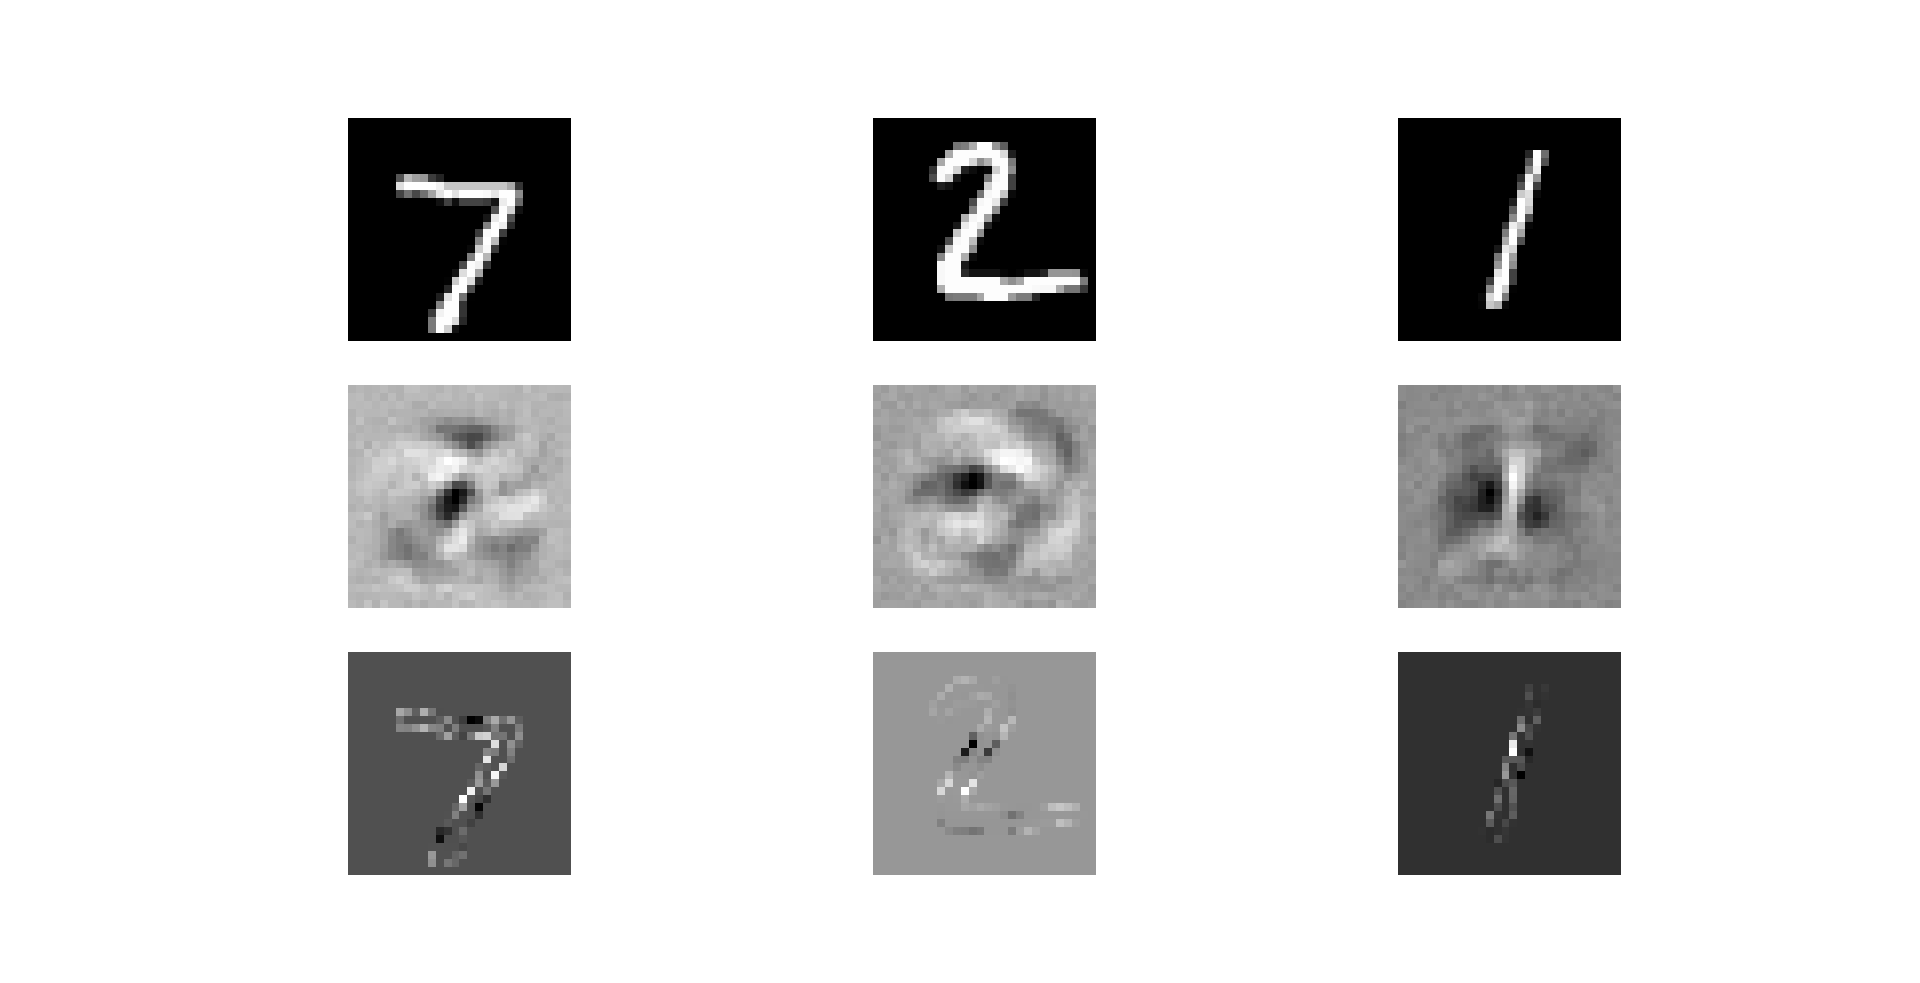
\includegraphics[width=\linewidth]{shapeshift.png}
	\caption{شکل و ماهیت حملات قبل و پس از تغییر توابع پایه‌ی ورودی. ردیف بالا مثال‌های طبیعی، ردیف وسط شکل حمله در صورت استفاده از توابع پایه‌ی تک‌جمله‌ای و ردیف آخر ماهیت حمله در صورت استفاده از توابع پایه‌ی مثلثاتی را نشان می‌دهند.}
	\label{fig:shape}
\end{figure}

نکته‌ی دیگری که در شکل دیده می‌شود، مشابه بودن رفتار حمله در انتخاب جهت اختلال خصمانه است. با کمی دقت، به نظر می‌رسد پیکسل‌هایی که در دو حالت مشترک هستند، رفتار مشابهی نیز از خود نشان می‌دهند و در هر دو حالت مکان پیکسل در تصویر  شدت و علامت آن را تعیین می‌کند. این موضوع با نتیجه‌ای که در \cite{goodfellow2014explaining} در مورد اهمیت جهت ورودی به دست آمده سازگاری دارد.

\section{جمع‌بندی}
در این مقاله دیدگاه جدیدی را در مورد چگونگی به وجود آمدن مثال‌های خصمانه و انتقال‌پذیری آنها در شبکه‌های عصبی را ارائه دادیم. طبق دیدگاه جدید، وجود مثال‌های خصمانه اثر جانبی همگرایی نقطه‌ای شبکه‌های عصبی بر روی مثال‌های طبیعی و انتقال‌پذیری آنها نتیجه‌ی همگرایی فرآیند آموزش به میانگینی از توابع درون‌یاب مثال‌های طبیعی و منظم بودن فاصله‌ی بین این مثال‌ها در نظر گرفته می‌شود. طبق نظریه‌ی تقریب جهانی، شبکه‌های عصبی توانایی تقریب زدن هر تابعی را دارند. با این حال، شواهد نشان می‌دهد در صورتی که مثال‌های طبیعی به صورت منظم در فضای ورودی توزیع شده باشند، یافتن طبقه‌بندی مناسب از میان تمامی طبقه‌بندهای نامناسب با چالش‌هایی، مستقل از مدل یادگیری، رو به رو است.

با در نظر گرفتن شباهات دیدگاه پیشنهادی و پدیده‌ی رونگه، روش‌های مقابله با مثال‌های خصمانه به دو گروه روش‌های کمترین مربعات و منظم‌سازی تقسیم می‌شوند. با این حال، در اجرای هر دوی این استراتژی‌ها مشکلاتی وجود دارد. در روش کمترین مربعات، نیاز به تولید مثال‌هایی خیالی داریم. از این لحاظ، آموزش خصمانه را می‌توان نوعی از روش‌های کمترین مربعات دانست. در مقابل، برای اجرای استراتژی منظم‌سازی نیاز به روش آموزشی خواهیم داشت که خروجی شبکه را در نقاطی ثابت نگه داشته و باقی درجات آزادی را برای ارضای هدف منظم‌سازی هزینه کند.

در ادامه، با تکیه بر دیدگاه پیشنهادی، کوانتیزه کردن ورودی را به عنوان یک استراتژی ارزان قیمت و موثر در کاهش اثرات مخرب پدیده‌ی مثال‌های خصمانه مورد بررسی قرار دادیم. شبکه‌های کوانتیزه شده در برابر حمله‌های بر پایه‌ی گرادیان ایمن هستند. در این شبکه‌ها، با احتمال قریب به یقین بردار گرادیان شبکه نسبت به ورودی برابر با صفر است. در نتیجه، مسئله‌ی یافتن مثال خصمانه برای این شبکه‌ها به یک مسئله‌ی بهینه‌سازی اعداد صحیح تبدیل می‌شود که حل آن نسبت به مسئله‌ی مشابه که بر روی اعداد حقیقی تعریف شده باشد سخت‌تر است. با این وجود، کوانتیزه کردن ورودی فقط مثال‌های خصمانه‌ی ناشی از درون‌یابی را از بین می‌برد و مثال‌های خصمانه‌ای که ناشی از ضعف برون‌یابی باشند را می‌توان همچنان با استفاده از روش‌های بهینه‌سازی اعداد صحیح و یا با استفاده از انتقال‌پذیری مثال‌های خصمانه به دست آورد. کوانتیزه کردن ورودی را می‌توان حالت خاصی از روش‌های مخفی کردن گرادیان برای ایمن‌سازی مدل‌های یادگیری ماشین در نظر گرفت.

دیدگاه پیشنهادی، برای کاربرد طبقه‌بندی تصاویر، روش مشخصی را برای مقاوم کردن شبکه نسبت به حملات خصمانه پیشنهاد می‌دهد. در این کاربرد، در صورتی که برچسب نقاط روی مرز دامنه‌ی ورودی را داشته باشیم، می‌توان برچسب نقاط فضای درونی ورودی را با تعمیم آنالتیک برچسب مرزها تعیین کرد. در نتیجه، در صورتی که ساختار شبکه یا روش آموزش را به گونه‌ای طراحی کنیم که شبکه‌ی یافت شده قید فوق را ارضا کند، بخش قابل توجهی از مثال‌های خصمانه از بین خواهند رفت. با این وجود، شواهد حاکی از آن است که مثال‌های خصمانه ممکن است به دلایل متفاوتی به وجود آیند. این موضوع نشان می‌دهد که روش‌های دیگری نیز برای بروز مثال‌های خصمانه، علاوه‌بر دیدگاه‌های مطرح شده، وجود دارند. خوشبختانه، می‌توان امیدوار بود که منظم‌سازی و افزایش مجموعه‌ی آموزشی تکنیک‌های کلی مبارزه با مثال‌های خصمانه باشند.

\setLTRbibitems
\bibliographystyle{plain}
\bibliography{refs.bib}

\end{document}